\begin{figure}[htbp]
\centering
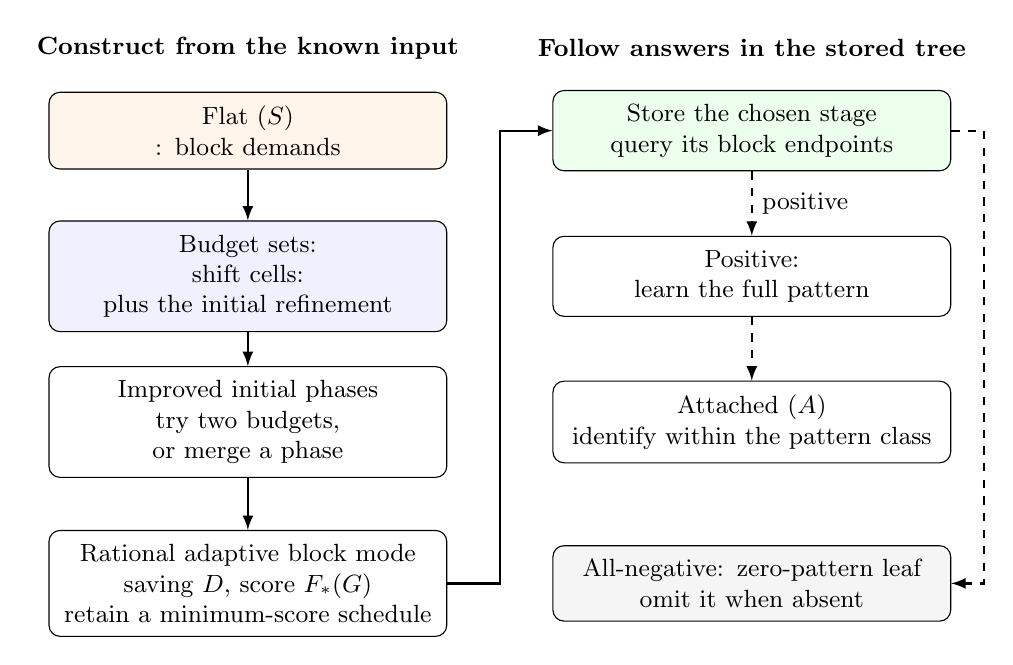
\begin{tikzpicture}[every node/.style={font=\small},
  box/.style={draw,rounded corners,align=center,inner sep=5pt,text width=4.7cm},
  arr/.style={-latex,thick},exec/.style={-latex,thick,dashed}]
  \node[font=\small\bfseries] at (-3.2,1.05) {Construct from the known input};
  \node[font=\small\bfseries] at (3.2,1.05) {Follow answers in the stored tree};
  \node[box,fill=orange!8] (hull) at (-3.2,0)
    {Flat \ExpectedTree$(S)$\\\HullData: block demands};
  \node[box,fill=blue!6] (covers) at (-3.2,-1.85)
    {Budget sets: \IntervalCover\\shift cells: \BatchOrders\\plus the initial refinement};
  \node[box] (variants) at (-3.2,-3.7)
    {Improved initial phases\\try two budgets, or merge a phase};
  \node[box] (score) at (-3.2,-5.75)
    {Rational adaptive block mode\\saving $D$, score $F_*(G)$\\retain a minimum-score schedule};
  \node[box,fill=green!7] (stored) at (3.2,0)
    {Store the chosen stage\\query its block endpoints};
  \node[box] (positive) at (3.2,-1.85)
    {Positive: \EndpointCode\\learn the full pattern};
  \node[box] (child) at (3.2,-3.7)
    {Attached \ExpectedTree$(A)$\\identify within the pattern class};
  \node[box,fill=gray!8] (zero) at (3.2,-5.75)
    {All-negative: zero-pattern leaf\\omit it when absent};
  \draw[arr] (hull) -- (covers);
  \draw[arr] (covers) -- (variants);
  \draw[arr] (variants) -- (score);
  \draw[arr] (score.east) -- (0,-5.75) -- (0,0) -- (stored.west);
  \draw[exec] (stored) -- node[right]{positive} (positive);
  \draw[exec] (positive) -- (child);
  \draw[exec] (stored.east) -- (6.15,0) -- (6.15,-5.75)
    -- (zero.east);
\end{tikzpicture}
\caption{The improved polynomial expected-depth procedure, including
the two-budget family of Algorithm~\ref{alg:two-phase-family}. The shift
cells include the refinement \eqref{eq:initial-shift-refinement}. Solid
arrows are construction-time data flow, computed from the supplied incidence
table and rational priors. Dashed arrows show how the unknown hypothesis
traverses the resulting tree; endpoint decoders and recursive children
are already constructed. Adaptive modes choose whether the first
positive block stops early or queries both endpoints. The certificate's
mixture is used in the proof of the bound, not to randomize execution.}
\label{fig:expected-procedure-flow}
\end{figure}

